\documentclass[a4paper, 10pt, fleqn]{article}

\usepackage[utf8]{inputenc}
\usepackage[T1]{fontenc}
\usepackage{textcomp}
\usepackage{lmodern}
\usepackage[ngerman]{babel}
\usepackage{tocbibind}
\usepackage{enumerate}
\usepackage{xcolor}
\usepackage{pdfpages}
\usepackage{amsmath}
\usepackage{graphicx}
\usepackage{geometry}
\usepackage{scrpage2}
\usepackage{lastpage}
\usepackage[hyphens]{url}
\usepackage{hyperref}
\usepackage{listings}
\usepackage{float}
\restylefloat{figure}
\lstset{language=[ansi]C++}

\newcommand{\code}[1]{\texttt{#1}}

\renewcommand*{\listoffigures}{%
  \begingroup
  \tocchapter
  \tocfile{\listfigurename}{lof}
  \endgroup
}

\geometry{left=3cm, top=3cm, bottom=3cm, right=2cm}

\hypersetup{
    colorlinks,
    linkcolor=black,
    citecolor=black,
    urlcolor=black
}

\pagestyle{scrheadings}
\ihead{PREN1 Gruppe 39}\ohead{Gesamtkonzept} 
\ifoot{\today} \ofoot{Seite \thepage\ von {\hypersetup{linkcolor=black}\pageref{LastPage}}}

% Einrücken zu Beginn von neuem Absatz unterdrücken
\setlength{\parindent}{0pt}


\begin{document}
% !TEX root = Dokumentation.tex
\begin{titlepage}   

\begin{center}
\textsc{\Large PREN Team 39}\\[0.5cm]

% Title
\newcommand{\HRule}{\rule{\linewidth}{0.5mm}}
\HRule \\[0.4cm]
{ \huge \bfseries GüselStar XXI}\\[0.4cm]
{ \LARGE \bfseries Gesamtkonzept}\\[0.4cm]
\HRule \\[1.5cm]

% Unterer Teil der Seite
{\large Horw, \today}

\begin{figure}[H]%Position festigen
\centering
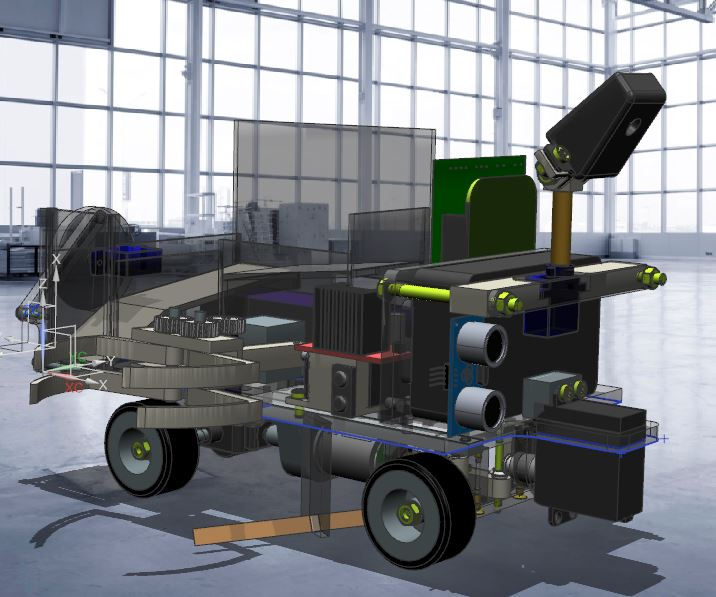
\includegraphics[width=0.7\textwidth]{03_Loesungskonzept/pictures/Tietelbild1.JPG}
\label{fig:activityRoute}
\end{figure}
% Author and supervisor
\begin{minipage}{0.4\textwidth}
\begin{flushleft} \large
\emph{Autoren:}\\
Patrizio Brantschen\\
Stefan Häfliger\\
Tobias Kreienbühl\\
Joël Meloni\\
Silvan Ritz\\
Lars Walther\\
\end{flushleft}
\end{minipage}
\hfill
\begin{minipage}{0.4\textwidth}
\begin{flushright} \large
\emph{Supervisor:} \\
Jürg Habegger
\end{flushright}
\end{minipage}
\large
\vfill
TA.BA\_PREN2.F1601 \\
Hochschule Luzern Technik \& Architektur

\end{center}

\end{titlepage}
\tableofcontents
\clearpage
% !TEX root = Dokumentation.tex
\section{Projektmanagement}

% !TEX root = Dokumentation.tex
\subsection{Team}

\large
\textbf{Maschinenbau}
\begin{table}[H]
\begin{tabular}{p{0.3\textwidth}p{0.3\textwidth}}	
	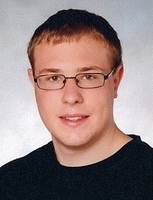
\includegraphics[width=0.25\textwidth]{./04_Projektmanagement/fig/stefanhaefliger.jpg}	&		
\includegraphics[width=0.25\textwidth]{./04_Projektmanagement/fig/joelmeloni.jpg} 
	\\
	\textbf{Stefan Häfliger} & 	
	\textbf{Joël Meloni}
	\\
	Beladen und Entladen &
	Chassis und Lenkung
\end{tabular}
\end{table}

\large
\textbf{Elektrotechnik}
\begin{table}[H]
\begin{tabular}{p{0.3\textwidth}p{0.3\textwidth}}	
	
\includegraphics[width=0.25\textwidth]{./04_Projektmanagement/fig/silvanritz.jpg}	&			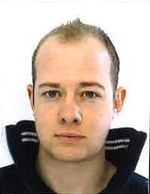
\includegraphics[width=0.27\textwidth]{./04_Projektmanagement/fig/larswalther.jpg} 
	\\
	\textbf{Silvan Ritz} & 	
	\textbf{Lars Walther}
	\\
	Servos, Sensoren und Freescale-Board &
	Energieversorgung und Antrieb
\end{tabular}
\end{table}

\newpage
\large
\textbf{Informatik}
\begin{table}[H]
\begin{tabular}{p{0.3\textwidth}p{0.3\textwidth}p{0.3\textwidth}}	
	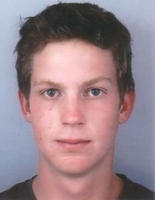
\includegraphics[width=0.26\textwidth]{./04_Projektmanagement/fig/patriziobrantschen.jpg}	&	
\includegraphics[width=0.24\textwidth]{./04_Projektmanagement/fig/adrianwuersch.jpg} &
	
\includegraphics[width=0.25\textwidth]{./04_Projektmanagement/fig/tobiaskreienbuehl.jpg} 
	\\
	\textbf{Patrizio Brantschen} & 	
	\textbf{Adrian Würsch} &
	\textbf{Tobias Kreienbühl}
	\\
	Objekterkennung und Rechtsvortritt &
	Schnittstellen und Dokumentation &
	Fahrbahnerkennung und Mini-Computer
\end{tabular}
\end{table}
\normalsize








% !TEX root = Dokumentation.tex
\subsection{Zeitplanung}



% !TEX root = Dokumentation.tex
\subsection{Risikomanagement}
Die Risiken, die während der Projektdurchführung entstehen könnten, sind im Folgenden aufgelistet. Um zu wissen, wie hoch ein Risiko eingeschätzt werden muss wurde eine Grafik erstellt. Zu jedem Risiko sind auch Massnhamen aufgelistet, welche im Eintrittsfall unternommen werden können. \\

\begin{figure}[H]%Position festigen
\centering
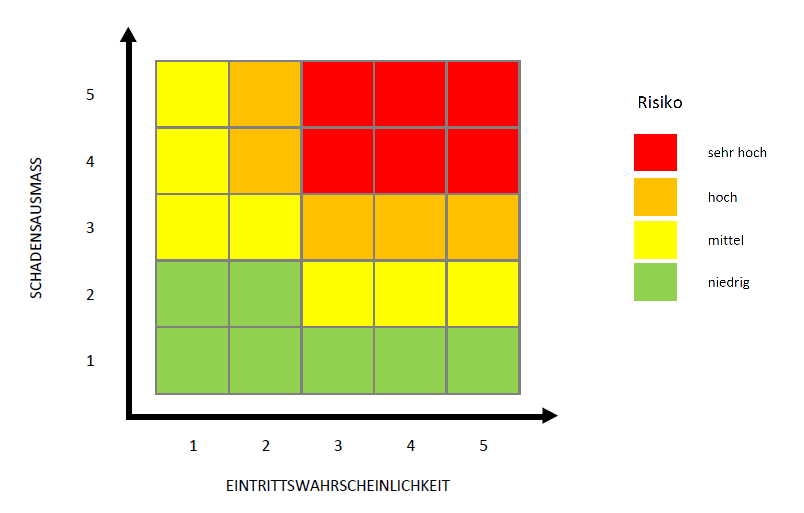
\includegraphics[width=0.8\textwidth]{Images/risikomatrix.png}
\caption{Risikomatrix}
\label{fig:Risikomatrix}
\end{figure}

\subsubsection{Risiken im Team}
\begin{table}[H]
\begin{tabular}{|p{0.3\textwidth}|p{0.2\textwidth}|p{0.2\textwidth}|p{0.2\textwidth}|}\hline
	
	\textbf{Risiko}	& 	\textbf{Wahrscheinlichkeit} & \textbf{Schadensausmass}  & \textbf{Massnahmen} \\\hline
	

	Mitglied verlässt das Team	&	1	&	4	&	Neuverteilung der Arbeiten \\\hline
	Unzuverlässigkeit eines Teammitglieds	&	2	&	3-4	&	 Absprache im Team, um eine Lösung zu finden  \\\hline
	Unstimmigkeiten unter den Teammitgliedern	& 	3	&	4	& Absprache im Team, um eine Lösung zu finden, evtl. auch Rat von Supervisor einholen.  \\\hline
	Mitglied überlastet	&	4	&	3	&	Neuverteilung der Arbeiten \\\hline
	Kommunikations-probleme	&	4	&	3	&	verbessert Absprachen, Frequenz der Sitzungen erhöhen \\\hline
	Fehlende fachliche Kompetenz eines Mitglieds	&	2	&	2	&	Neuverteilung der Arbeiten \\\hline
	Fehlende soziale Kompetenz eines Mitglieds	&	1	&	3	&	Absprache im Team, um eine Lösung zu finden \\\hline
\end{tabular}\\
\end{table}

\subsubsection{Risiken Projektmanagement}
\begin{table}[H]
\begin{tabular}{|p{0.3\textwidth}|p{0.2\textwidth}|p{0.2\textwidth}|p{0.2\textwidth}|}\hline
	
	\textbf{Risiko}	& 	\textbf{Wahrscheinlichkeit} & \textbf{Schadensausmass}  & \textbf{Massnahmen} \\\hline
		Missverständnisse bei den Anforderungen	&	3-4	&	3	& Absprache mit Supervisor  \\\hline
	Ineffizientes Arbeiten	&	3-4	&	2-3	& Neuorganisierung der Vorgehensweise  \\\hline
	
	Überschreitung des Budgets	&	1	&	4	& Absprache mit Supervisor  \\\hline
\end{tabular}\\
\end{table}

\subsubsection{Risiken bei der Realisierung}
\begin{table}[H]
\begin{tabular}{|p{0.3\textwidth}|p{0.2\textwidth}|p{0.2\textwidth}|p{0.2\textwidth}|}\hline
	
	\textbf{Risiko}	& 	\textbf{Wahrscheinlichkeit} & \textbf{Schadensausmass}  & \textbf{Massnahmen} \\\hline
	
	Idee funktioniert nicht wie gewünscht	&	2	&	4 & neue Ideenfindung, Rat einholen  \\\hline
	Eingekaufte Komponente erfüllt Anforderung nicht	&	2	&	5	& andere Komponente einkaufen  \\\hline
		Projekt-anforderungen sind nicht erfüllt	&	1	&	5	&  Anpassungen planen \\\hline
\end{tabular}\\
\end{table}

\subsubsection{Andere Risiken}
\begin{table}[H]
\begin{tabular}{|p{0.3\textwidth}|p{0.2\textwidth}|p{0.2\textwidth}|p{0.2\textwidth}|}\hline
	
	\textbf{Risiko}	& 	\textbf{Wahrscheinlichkeit} & \textbf{Schadensausmass}  & \textbf{Massnahmen} \\\hline
	
	Lange Lieferzeiten bei Bestellungen	&	3	&	2	& andere Arbeiten aufnehmen, früher bestellen  \\\hline
	Github fällt aus	&	1	&	4	& Lokal weiterarbeiten  \\\hline
\end{tabular}\\
\end{table}


% !TEX root = Dokumentation.tex
\subsection{Budgetplanung}

% !TEX root = Dokumentation.tex
\subsection{Projektunterstützung}
Während der Durchführung des Projekts soll der administrative Aufwand möglichst klein gehalten werden können. Weiter sollen alle Projektmitglieder gleichzeitig an der Software weiterentwickeln oder an der Dokumentation weiterschreiben können. Darum wird auf diverse Software-Produkte und -Systeme zurückgegriffen, die sich in der Praxis bewährt haben.
%
\subsubsection{Software}
\begin{table}[H]
\begin{tabular}{|p{0.3\textwidth}|p{0.64\textwidth}|}\hline
%	
Kommunikation	&	E-Mail, Whatsapp \\\hline
Dokumenterstellung & LaTeX\\\hline
Versionsverwaltungssoftware & Git \\\hline
Filehosting-Dienst & GitHub \\\hline
CAD-Software & NX\\\hline
Entwicklungsumgebung	& Eclipse, Kinetis Design Studio \\\hline
%
\end{tabular}
\end{table}
LaTeX ermöglicht es, die gesamte Dokumentation in mehrere Teildokumente zu unterteilen. All diese Dokumente sind in GitHub eingecheckt. Somit wird sichergestellt, dass mehrere Teammitglieder zur selben Zeit an der Dokumentation arbeiten können und dabei möglichst wenig Konflikte entstehen. Weiter wird auf dem selben Git-Repository auch der Quellcode der Software abgelegt. \\
\subsubsection{Aufgabenverteilung}
Um die Aufgabenverteilung festzuhalten wurde ein Scrum-Board erstellt. Darauf sind alle Team-Mitglieder aufgelistet. Zudem sind, wie bei Scrum üblich, die drei Zustände \glqq ToDo\grqq, \glqq Doing\grqq \ und \glqq Done\grqq \ definiert.
\begin{figure}[H]%Position festigen
\centering
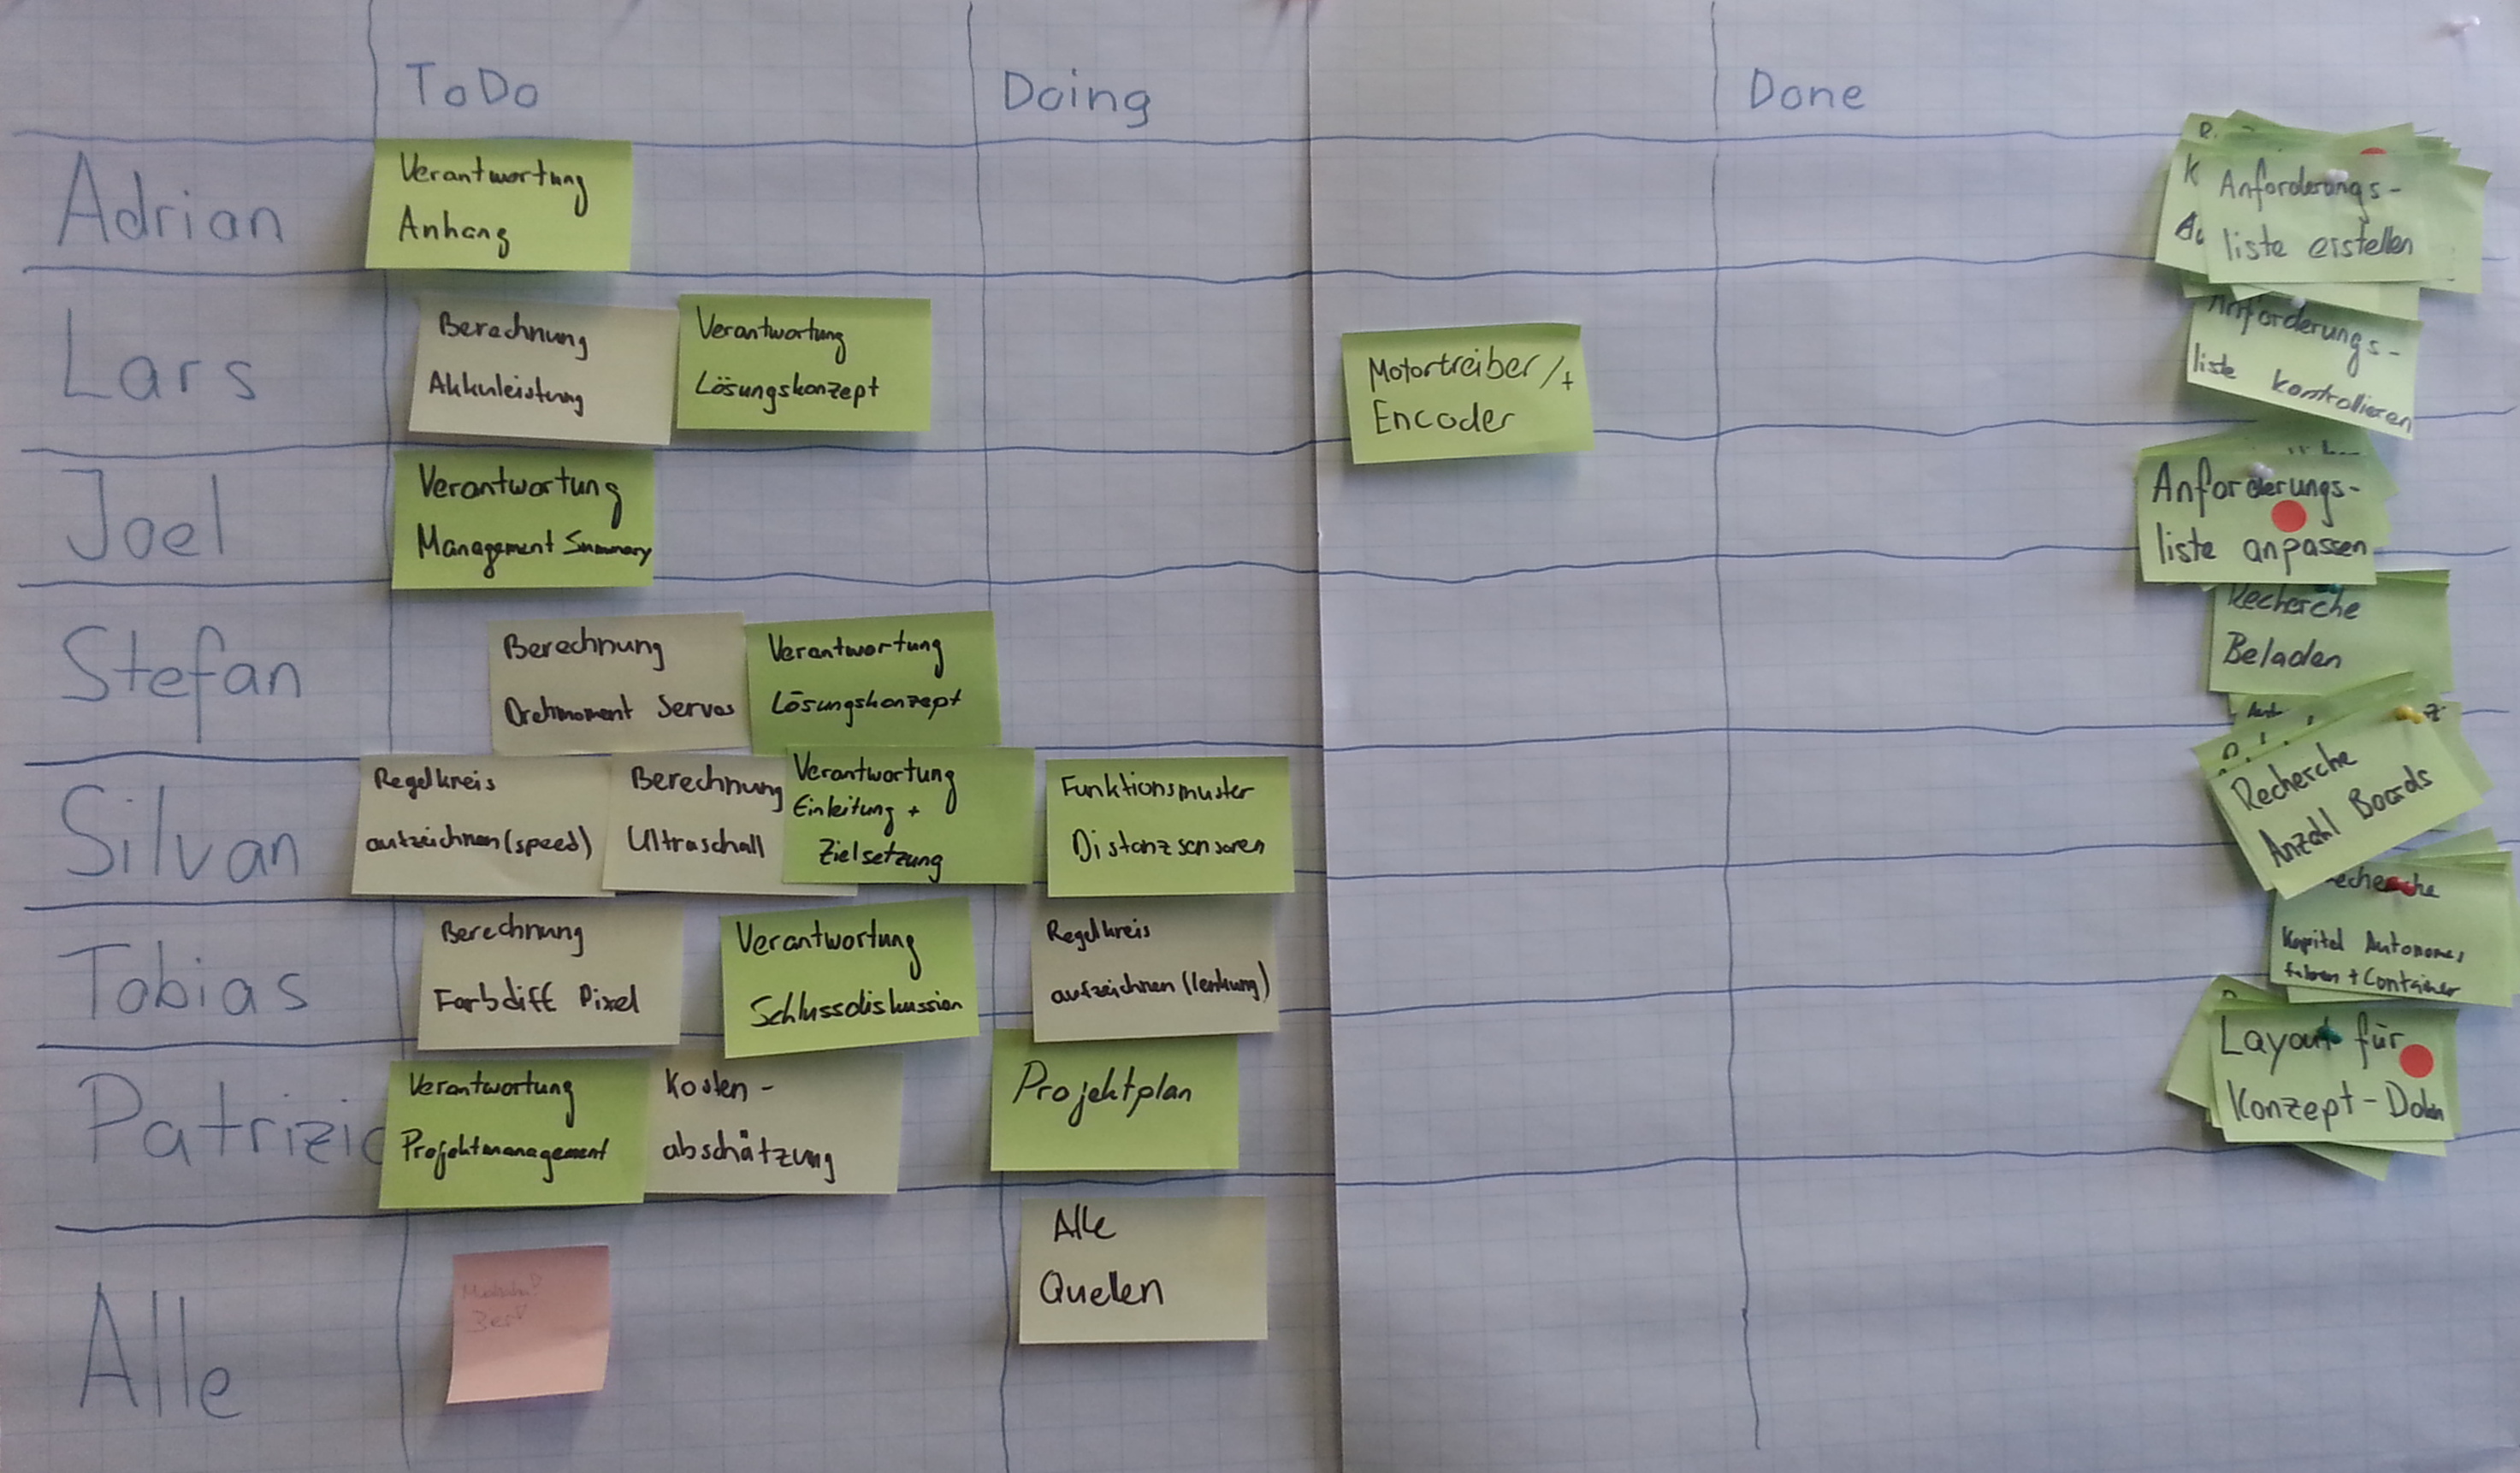
\includegraphics[width=0.8\textwidth]{04_Projektmanagement/fig/scrumBoard.jpg}
\caption{Scrum-Board}
\label{fig:scrumBoard}
\end{figure}
\end{document}